\documentclass[tikz,border=5pt]{standalone}
\usepackage{luatexja}
\usepackage[hiragino-pron]{luatexja-preset}
\usepackage{amsmath,amssymb}
\usepackage{pgfplots}
\pgfplotsset{compat=1.18}
\usetikzlibrary{arrows.meta,calc,decorations.markings,patterns,positioning}

% Common styles
\tikzset{
  axis/.style={-{Stealth[length=6pt]}, thick},
  curve/.style={thick, red},
  dashed curve/.style={thick, dashed, blue},
  dot/.style={circle, fill, inner sep=1.5pt},
  open dot/.style={circle, draw, fill=white, inner sep=1.5pt},
}

\begin{document}
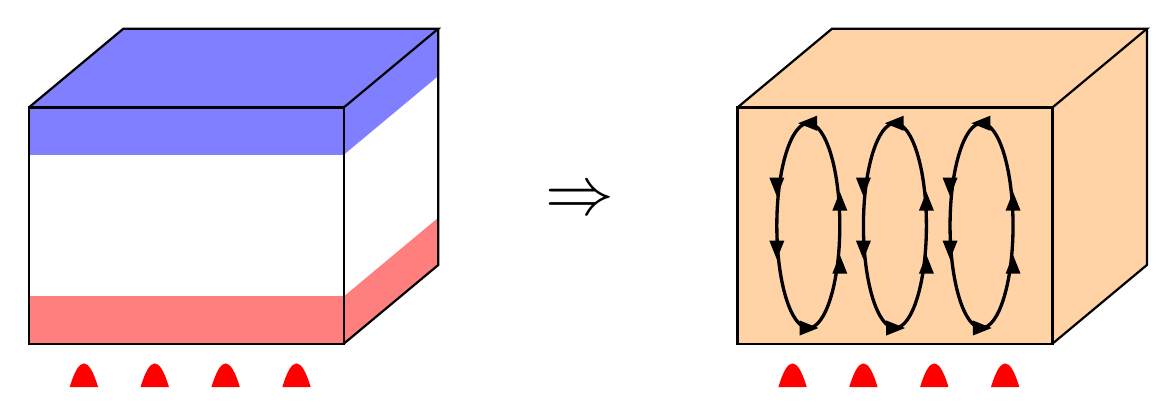
\begin{tikzpicture}[>=Stealth, thick]

  % Perspective offset for 3D
  \pgfmathsetmacro{\dx}{1.2}
  \pgfmathsetmacro{\dy}{1.0}

  % === Left box: before heating (stratified) ===
  \begin{scope}
    % Red band (bottom of front face)
    \fill[red, opacity=0.5] (0,0) rectangle (4,0.6);
    % Red band (bottom of right face)
    \fill[red, opacity=0.5] (4,0) -- (4+\dx,\dy) -- (4+\dx,\dy+0.6) -- (4,0.6) -- cycle;

    % Blue band (top of front face)
    \fill[blue, opacity=0.5] (0,3-0.6) rectangle (4,3);
    % Blue band (top face)
    \fill[blue, opacity=0.5] (0,3) -- (\dx,3+\dy) -- (4+\dx,3+\dy) -- (4,3) -- cycle;
    % Blue band (top of right face)
    \fill[blue, opacity=0.5] (4,3-0.6) -- (4+\dx,3+\dy-0.6) -- (4+\dx,3+\dy) -- (4,3) -- cycle;

    % Box edges
    \draw (0,0) rectangle (4,3);
    \draw (0,3) -- (\dx,3+\dy) -- (4+\dx,3+\dy) -- (4,3);
    \draw (4,0) -- (4+\dx,\dy) -- (4+\dx,3+\dy);

    % Flames below
    \foreach \x in {0.7, 1.6, 2.5, 3.4} {
      \fill[red] (\x-0.18,-0.55) .. controls (\x-0.06,-0.15) and (\x+0.06,-0.15) .. (\x+0.18,-0.55) -- cycle;
    }
  \end{scope}

  % === Arrow ===
  \node[font=\Huge] at (7, 1.8) {$\Rightarrow$};

  % === Right box: after convection (well-mixed) ===
  \begin{scope}[xshift=9cm]
    % Orange fill (front face)
    \fill[orange, opacity=0.35] (0,0) rectangle (4,3);
    % Orange fill (right face)
    \fill[orange, opacity=0.35] (4,0) -- (4+\dx,\dy) -- (4+\dx,3+\dy) -- (4,3) -- cycle;
    % Orange fill (top face)
    \fill[orange, opacity=0.35] (0,3) -- (\dx,3+\dy) -- (4+\dx,3+\dy) -- (4,3) -- cycle;

    % Box edges
    \draw (0,0) rectangle (4,3);
    \draw (0,3) -- (\dx,3+\dy) -- (4+\dx,3+\dy) -- (4,3);
    \draw (4,0) -- (4+\dx,\dy) -- (4+\dx,3+\dy);

    % Three convection cells (vertical ellipses with arrows)
    \foreach \cx in {0.9, 2.0, 3.1} {
      \draw[very thick] (\cx, 1.5) ellipse (0.4 and 1.3);
      % Left side: arrows pointing up
      \draw[semithick, fill=black] (\cx-0.4, 1.9) -- ++(-.08,.2) -- ++(.16,0) -- cycle;
      \draw[semithick, fill=black] (\cx-0.4, 1.1) -- ++(-.08,.2) -- ++(.16,0) -- cycle;
      % Right side: arrows pointing down
      \draw[semithick, fill=black] (\cx+0.4, 1.1) -- ++(-.08,-.2) -- ++(.16,0) -- cycle;
      \draw[semithick, fill=black] (\cx+0.4, 1.9) -- ++(-.08,-.2) -- ++(.16,0) -- cycle;
      % Top: arrow pointing right
      \draw[semithick, fill=black] (\cx-0.10, 2.8) -- ++(.2,.08) -- ++(0,-.16) -- cycle;
      % Bottom: arrow pointing left
      \draw[semithick, fill=black] (\cx+0.10, 0.2) -- ++(-.2,-.08) -- ++(0,.16) -- cycle;
    }

    % Flames below
    \foreach \x in {0.7, 1.6, 2.5, 3.4} {
      \fill[red] (\x-0.18,-0.55) .. controls (\x-0.06,-0.15) and (\x+0.06,-0.15) .. (\x+0.18,-0.55) -- cycle;
    }
  \end{scope}

\end{tikzpicture}
\end{document}
